\documentclass[a4]{article}
\usepackage[utf8]{inputenc}
\usepackage[brazil]{babel}
\usepackage{url}
\usepackage{tabularx}
\usepackage{palatino}
\usepackage{hyperref}
\usepackage{graphicx}
\usepackage{float}
\usepackage[margin=2cm]{geometry}

\title{\textbf{Lista 2 de IPN0007 - Redes Neurais na Engenharia Nuclear}}
\author{
    \textbf{Aluno:} Luís Felipe de Melo  \\
    \textbf{Número USP:} 9297961
    }
\date{}
\begin{document}
\maketitle

\section*{Exercício 1}

A apresentação do Perceptron de Rosenblatt, em 1958. 

\section*{Exercício 2}

O Perceptron de Rosenblatt era uma RNA de apenas uma camada. Ele tinha 400 células fotoelétricas que recebiam estímulos óticos e eram ligados a processadores (unidades associativas). O processamento acontecia, então, como no Neurônio de McCulloch-Pitts: produto escalar do vetor de entrada por um vetor de pesos, cujo resultado passa por uma função limiar e resulta na saída.

\section*{Exercício 3}

As RNA têm seu desenvolvimento pautado por dois tipos de ciclos: de ceticismo e de entusiasmo.

\begin{itemize}
	\item Nos de ceticismo, a pesquisa possui menos sucesso, em geral, causada por algum problema técnico, ou porque existe menos interesse. São alguns desses ciclos:
	\begin{itemize}
		\item De 1949 até 1958: a eletrônica não era confiável para a implantação de neurônios artificiais.
		\item De 1969 até 1982: percebeu-se que havia um problema de separação linear, já que uma camada não conseguia separar dados além disso.
	\end{itemize}
	\item Nos de entusiasmo, ocorre o contrário, o interesse está no auge e a tecnologia auxilia nos desenvolvimentos. São exemplos:
	\begin{itemize}
		\item De 1958 até 1969: o desenvolvimento do Perceptron de Rosenblatt e do ADALINE fez o interesse pela área aumentar.
		\item De 1982 até 1998: a invenção e reinvenções do algoritmo de retro-propagação se tornaram base para diversos estudos na área. Além disso, foram introduzidas as redes convolutivas.
		\item De 1998 até 2010: período de incubação, onde as pesquisas se aprofundaram no desenvolvimento de conceitos de \textit{Deep Learning}.
	\end{itemize}
\end{itemize}

\section*{Exercício 4}

Um neurônio de McCullogh consegue fazer apenas separações lineares, como as mostradas abaixo.

\begin{figure}[H]
	\centering
	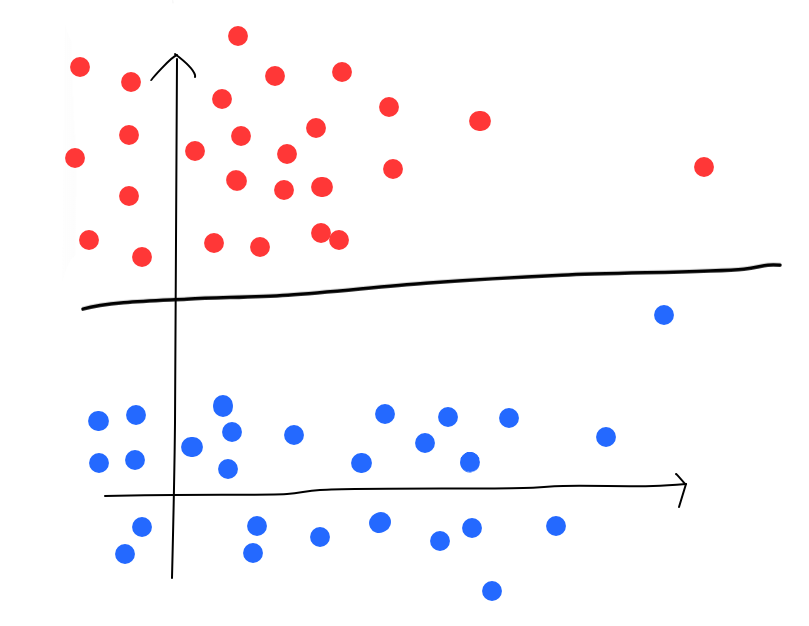
\includegraphics[width=0.45\linewidth]{esquema1}
	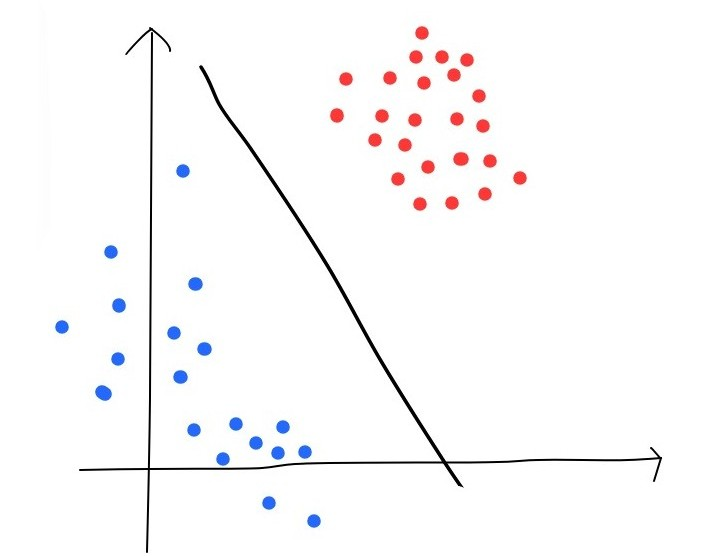
\includegraphics[width=0.45\linewidth]{esquema2}
	\caption{Exemplos de dados linearmente separáveis}
\end{figure}

\section*{Exercício 5}
 
\section*{Exercício 6}

A diferença entre o perceptron e o ADALINE é que o erro deste segundo é baseado na saída linear, e não na saída binária.

\section*{Exercício 7}

O limiar é um valor que define a ativação do neurônio ou não, de acordo com o valor de saída. Por exemplo, se a saída é maior que o limiar, o neurônio é ativado (fornece uma resposta positiva).

\section*{Exercício 8}

Um padrão, na área de RNAs, é obtido através dos dados e pode representar um estado, uma condição, uma característica, entre outros, que é o que se deseja aprender para responder o problema.

\section*{Exercício 9}

Redes alimentadas adiante redes com realimentação e mapas auto-organizáveis.

\section*{Exercício 10}



\end{document}
